% !TEX TS-program = pdflatex
% !TEX encoding = UTF-8 Unicode

% This is a simple template for a LaTeX document using the "article" class.
% See "book", "report", "letter" for other types of document.

\documentclass[12pt]{article} % use larger type; default would be 10pt

\usepackage[utf8]{inputenc} % set input encoding (not needed with XeLaTeX)

%%% Examples of Article customizations
% These packages are optional, depending whether you want the features they provide.
% See the LaTeX Companion or other references for full information.

%%% PAGE DIMENSIONS
\usepackage{geometry} % to change the page dimensions
\geometry{letterpaper,margin=1in} % or letterpaper (US) or a5paper or....
% \geometry{margin=2in} % for example, change the margins to 2 inches all round
% \geometry{landscape} % set up the page for landscape
%   read geometry.pdf for detailed page layout information

\usepackage{graphicx} % support the \includegraphics command and options

% \usepackage[parfill]{parskip} % Activate to begin paragraphs with an empty line rather than an indent

%%% PACKAGES
\usepackage{bbm}
\usepackage{booktabs} % for much better looking tables
\usepackage{array} % for better arrays (eg matrices) in maths
\usepackage{paralist} % very flexible & customisable lists (eg. enumerate/itemize, etc.)
\usepackage{verbatim} % adds environment for commenting out blocks of text & for better verbatim
%\usepackage{subfig} % make it possible to include more than one captioned figure/table in a single float
\usepackage{caption}
\usepackage[singlelinecheck=on,labelformat=simple]{subcaption}
	\renewcommand\thesubfigure{(\alph{subfigure})}
	\renewcommand\thesubtable{(\alph{subtable})}
\usepackage{hyperref}
  \hypersetup{colorlinks   = true, urlcolor= blue, linkcolor=black,citecolor=blue}
\usepackage{natbib}
\usepackage[section]{placeins} %keep figure in section
\usepackage{setspace} %for double space
\usepackage{amsmath}
\usepackage{amsfonts}
\newcommand{\ar}[1]{\text{ar}\left( #1 \right)}

%%% HEADERS & FOOTERS
\usepackage{fancyhdr} % This should be set AFTER setting up the page geometry
\pagestyle{fancy} % options: empty , plain , fancy
\renewcommand{\headrulewidth}{0pt} % customise the layout...
\lhead{}\chead{}\rhead{}
\lfoot{}\cfoot{\thepage}\rfoot{}

%%% SECTION TITLE APPEARANCE
\usepackage{sectsty}
\allsectionsfont{\sffamily\mdseries\upshape} % (See the fntguide.pdf for font help)
% (This matches ConTeXt defaults)

%%% ToC (table of contents) APPEARANCE
\usepackage[nottoc,notlof,notlot]{tocbibind} % Put the bibliography in the ToC
\usepackage[titles,subfigure]{tocloft} % Alter the style of the Table of Contents
\renewcommand{\cftsecfont}{\rmfamily\mdseries\upshape}
\renewcommand{\cftsecpagefont}{\rmfamily\mdseries\upshape} % No bold!

%%% END Article customizations

%%% The "real" document content comes below...
\graphicspath{{./images/}}
\begin{document}
\begin{titlepage}
	
	\begin{center}
		\vspace{10cm}
		
		% Upper part of the page
		
\includegraphics[width=.5\textwidth]{./images/primarylogo}\\[3cm]    
		
		\normalsize EE 227C\\
		\textsc{\large Convex Optimization}\\[1cm]		
		
		% Title
		\hrule 
		\vspace{1 cm}
		{ \Large \textbf{A Platform for Solving Constraint Satisfaction Problems via Semidefinite Programming}\\[0.5cm]
			\vspace{0.5 cm}
			\hrule
			\vspace{1.5 cm}
			
			% Author and supervisor
			\begin{minipage}[t]{0.4\textwidth}
				\begin{flushleft} \large
					\emph{Authors:}\\
					\vspace{0.7ex}
					Riley \textsc{Murray} \\
					Paul \textsc{Anderson}
					
				\end{flushleft}
			\end{minipage}
			\begin{minipage}[t]{0.4\textwidth}
				\begin{flushright} \large
					\emph{Instructor:} \\
					\vspace{0.7ex}
					Benjamin \textsc{Recht}\\[0.3 cm]
				\end{flushright}
			\end{minipage}
			\vfill 
			% Bottom of the page
			University of California, Berkeley\\[.5cm]
			\large \today}
		
	\end{center}
	
\end{titlepage}

\section*{Abstract}

A Constraint Satisfaction Problem (CSP) is a discrete optimization problem consisting of a set of variables (which take on values in a finite domain) and a set of constraints (indicator functions defined on a subset of variables of some specified cardinality). The objective in a CSP is to assign each variable a value in the domain so that the largest number of constraints are satisfied.

CSP's subsume a wide range of fundamental combinatorial optimization problems, including Max k-SAT, graph coloring (approximately defined), and Unique Games.

Significant effort has been dedicated to developing approximation algorithms for CSP's. The most general of these algorithms involve solving a canonical SDP relaxation of the CSP (called ``Basic SDP" \cite{raghavendra2008optimal}) and use extremely sophisticated post-processing of SDP vectors to determine an assignment of variables. Unfortunately, as was shown in \cite{dwivedi2015introduction}, these algorithms require impossibly powerful machines.

In this work, we deploy approximation algorithms rooted in theory but driven by practical considerations to approximate CSP's with the machines of today and the near future. We developed a Matlab-based software package for CSP's. This package takes a CSP object, computes the Basic SDP relaxation of the problem and solves it using SDPNAL+, and then uses heuristic methods to turn the SDP solution into an assignment of variables for the CSP.  The assignment heuristics used are SDP vector clustering and an approximation of the Variable Folding Method. We tested this software package on two CSP's: a graph-coloring problem, and pigeonhole problems of various sizes. Our approximation of the Variable Folding Method is found to perform best, closely approximating or matching the optimal solution while reducing the number of variables by over 80\% in large problems. We conclude with a discussion of issues related to scaling and applications in Ramsey Theory.

\section{Introduction}

CSP's are concerned with a set of variables, $V$, taking values in a finite domain $D$ with consideration to a set of constraints $C$. We emphasize that while most optimization literature considers``constraints'' inviolable, this is not the case for CSP's. In fact, it is the \textit{objective} of a CSP to satisfy as many of constraints as possible, and an optimal solution may well only satisfy a small portion of these constraints. We say that a CSP is \textit{satisfiable} if there exists an assignment of variables for which all constraints are satisfied. Inviolable constraints do exist within the CSP framework, but those constraints are \textit{only} that each $v \in V$ takes a value in $D$. This established, we discuss the constraints of a CSP in more detail. 

Let $\Omega_D^k$ be the set of all functions on $k$ or fewer variables (each taking values in $D$) with range $\{ 0,1 \}$. A \textit{constraint} $C_i$ for a CSP over variable set $V$ is any function in $\Omega_D^k$ defined on $S \subset V : |S| \leq k$. We refer to the $S \subset V$ as the \textit{scope} of the constraint, and refer to $|S|$ as the \textit{arity} of the constraint. The maximum arity of all constraints in a CSP is considered a fixed parameter (in the fixed-parameter tractability sense). In view of this, we simplify exposition by assuming that all constraints are of arity $k$.\footnote{Our software package for CSP approximation does not make this assumption.}

While the generality of this framework is useful, it can appear a bit opaque. To bring us back to more familiar territory, we can divide CSP's into well-known classes of problems by drawing the constraint functions from some $\Gamma \subset \Omega_D^k$.

\begin{center}
\begin{tabular}{c c c l}
\hline
k & D & $\Gamma$ & Problem \\
\hline
2  & \{0,1\} & $\{\neq\}$ & Max-Cut \\
3  & \{0,1\} & All disjunctions on $\leq $ 3 literals & Max 3-SAT \\
10 & \{0,1\} & $\neg$[All-Equal] & Finding Ramsey(5,5) \\
2  & \{0,1,...,q-1\} & $\{\neq\}$ & Graph Coloring \\
\hline
\end{tabular}
\end{center}

Significant effort has been dedicated to developing approximation algorithms for CSP's. The most general of these algorithms involve solving a canonical SDP relaxation of the CSP ``Basic SDP" \cite{raghavendra2008optimal}. This report is concerned with constructing, solving, and rounding solutions for the Basic SDP relaxation of a CSP. Along the way, we present new links between hardness-of-approximation (in the computer algorithms sense) and Ramsey Theory.


\subsection{Our Contributions}
 
Our primary contribution is the development of a Matlab based software package for working with CSP's. Our codes deal with the Basic SDP relaxation for a CSP, rounding of the associated SDP solutions, and solving small scale CSP's exactly via integer programming. The software package has the following capabilities.

\begin{enumerate}
\item Given a Matlab CSP object, we can efficiently construct SDP input parameters in the format used by SDPT3 ( a core routing in CVX and Yalmip) and SDPNAL+ ( a cutting edge solver capable of solving SDP's with $>$ 10 million linear equality constraints).

\item Given a Matlab CSP object, we can solve it to arbitrary accuracy with a MIP formulation via the Gurobi Optimization solver.

\item Given the solution to Basic SDP for a given CSP, we can return an assignment of variables for the CSP based on various heuristic adaptations of published (but impractical) algorithms.
\end{enumerate}
Our software package makes use of the Matlab CSP abstraction of \cite{dwivedi2015introduction}.

We address a variety of considerations for semidefinite programming at scale (particularly memory management and linearly independent constraint qualification), and we demonstrate how hardness-of-approximation relates to Ramsey Theory.


\section{CSP's for Ramsey Theory}
Ramsey theory is the study of combinatorial objects in which a certain amount of order must occur as the scale of the object becomes large \cite{rt}. The most well-known topic in Ramsey theory is that of Ramsey \textit{numbers}. Ramsey numbers deal with questions of the following form : 

\vspace{1em}
\noindent \textit{for fixed $n$ and $m$, what is the smallest $\alpha$ such that for \textit{any} 2-coloring of edges in $K_\alpha$, there necessarily exists a monochromatic clique of size $n$, or a monochromatic clique of size $m$?}
\vspace{1em}

This``smallest $\alpha$'' is referred to as ``Ramsey of $n,m$'', or simply $R(n,m)$. When $n = m$, we write $R(n)$.

Although it has been proven for any $n,m$ there \textit{exists} a finite $R(n,m)$ satisfying the requirements above, the exact values $R(n,m)$ are largely unknown. For example, $R(5)$ is only known to lay in $[43,49]$, and this has remained unchanged for the past 20 years \cite{rn}. We now turn to formulating a sequence of CSP's for which optimal solutions would determine $R(5)$, and for which approximate solutions may yield new bounds on the same.

Suppose we are interested in testing whether $R(5) \leq 48$. Construct the complete graph on 48 vertices, $K_{48}$, and for each edge in $K_{48}$ define a variable taking values in $\{\text{red},\text{blue}\}$ for our CSP. For every induced subgraph on 5 vertices, define a constraint with scope of the 5-choose-2 edges in this subgraph. Set the relation for this constraint as the not-all-equal operator. Stated in these terms, $R(5) \leq 48$ if and only if the optimal solution to this CSP satisfies less than 100\% of all constraints (i.e. if the CSP is ``not satisfiable'').

More generally, one can construct a CSP which asks whether $R(n) \leq L$ by identifying edge colors of $K_L$ with variables in our CSP, and by identifying edges of induced subgraphs on $n$ vertices as scopes for our constraints. In all cases, the relation on these variables is the not-all-equal operator. In all cases, $R(n) \leq L$ if and only if this CSP is not satisfiable.

Of course, our use of CSP's is posed as a decision problem in a way that could also be modeled with 3-SAT by introduction of appropriate helper variables. Our insight is that while SAT solvers try to find \textit{exact} solutions, algorithms in CSP literature are concerned with \textit{approximate} solutions, and approximate solutions can be used to bound optimal solutions. In particular, if the Basic SDP relaxation for a Ramsey CSP has optimal objective less than 1, then that CSP \textit{cannot} be satisfiable. 

Since the integrality gap of Basic SDP is quite possibly smallest-possible\footnote{In that there may not exist a mathematical programming relaxation of any subclass of CSP's for which the largest distance between a relaxation's objective and the true optimal objective is smaller than that of Basic SDP.} \cite{raghavendra2008optimal}, it is reasonable to use SDP relaxations for CSP's in the manner of one-sided hypothesis tests on Ramsey number bounds.

\section{An Overview of Basic SDP}

Basic SDP operates on a principle of consistency across local assignments. A local assignment for a constraint $C_i$ is a mapping $L_i$ from $S_i$ to $D^{k}$; there are $|D|^k$ such local assignments for each constraint. A collection of \textit{consistent} local assignments is any set of mappings $\mathfrak{L}$ such that for all $L_i, L_j \in \mathfrak{L}$ with $v \in S_i \cap S_j$, we have $L_i(v) = L_j(v)$.

Basic SDP introduces one variable for each local assignment of each constraint, and establishes coupling constraints between 

Basic SDP introduces one variable for each local assignment of each constraint $(y_i[L])$ and establishes coupling constraints between these variables. Basic SDP \cite{raghavendra2008optimal} is reproduced below, \emph{without} the usual scaling of the objective by $1/m$.

\begin{align}
\operatorname*{max}_{\substack{y \geq 0 \\  X \succeq 0}} ~ & ~ \sum\limits_{i:C_i\in C} \sum\limits_{L\in \mathcal{L}_i} R_i(L)y_i[L] \nonumber  \\
s.t. ~ & ~ \sum\limits_{L \in \mathcal{L}_i} y_i[L] = 1  \quad \forall i : C_i \in C \\
& ~ \sum\limits_{\substack{L \in \mathcal{L}_i \\ L(v)=\ell \\ L(v')=\ell '}} y_i[L] = X_{(v,\ell),(v',\ell')}  \quad \forall (v,\ell,v',\ell') : \exists C_i = (S_i, f_i) \text{ with } v,v' \in S_i \\
& ~ 0 \leq  X_{(v,\ell),(v',\ell')}  \leq \mathbbm{1}\{ v \neq v' \text{ or } \ell = \ell' \}
\end{align}

This SDP also has a probabilistic interpretation, if we made the following identifications:

\begin{equation}
X_{(v,\ell),(v',\ell')} = \mathbb{E}[I_v(\ell)I_{v'}(\ell')] = \mathbb{P}_{L\sim y_i}[L(v)=\ell, L(v')=\ell']
\end{equation}

\section{Rounding Schemes for Basic SDP (principled and heuristic)}


\subsection{The Variable Folding Method}

The Variable Folding Method (VFM) is a rounding scheme for Basic SDP introduced in \citet{raghavendra2009round}. At a high level, VFM performs a Cholesky (or LDL) factorization of the SDP matrix $X$, then projects the resulting SDP vectors onto a random subspace of dimension $\beta$. Once the SDP vectors are projected onto this random subspace, they are classified over an $\epsilon$-net of the unit ball in $\mathbb{R}^\beta$. Variables whose associated SDP vectors are classified in identical ways are merged, and a new CSP is defined in this variable-merging process. The new CSP is called a ``folding" of the original CSP and needs to be solved by an exact algorithm (we use Gurobi Optimization solver for this purpose). VFM completes by ``unfolding" the optimal assignment of variables for the folded CSP into an assignment of variables for the original CSP.

VFM is polynomial in that the folded CSP has a bounded number of variables, but this bound is impossibly large to be useful with today's computer systems \citep{dwivedi2015introduction}. We mitigate this issue by projecting onto an extremely small dimension ($\beta = 2$), and choosing $\epsilon$ for our $\epsilon$-net in a generous way.

\subsection{SDP Vector Clustering}

VFM has two computationally expensive operations (three if you count solving Basic SDP): (1) constructing an $\epsilon$-net of the unit ball in $\mathbb{R}^\beta$ for $\beta>>2$, and (2) solving a resulting CSP exactly. We have implemented a much simpler procedure that appeals to the notion that CSP variables with similar sets of SDP vectors can be lumped together as a single variable. Step 1: project SDP vectors onto a random subspace of any dimension $\geq |D|$. Step 2: assemble all SDP vectors associated with a CSP variable into a single vector. Step 3: cluster the resulting vectors into $|D|$ equivalence classes. Step 4: assign variables arbitrarily for symmetric CSP's (e.g. graph coloring) and test $|D|!$ assignments for asymmetric CSP's (e.g. 3-SAT).


\section{Practical Considerations in Solving Large SDP's}

SDPNAL+ \cite{yang2015sdpnal+, zhao2010newton} is a combination MATLAB / C implementation of a hybrid Newton Conjugate Gradient \& Alternating Direction Method of Multipliers solver for SDP's with bound constraints.

SDPNAL+ is not supported by any general purpose modeling language. As a result, we needed to build all constraint matrices directly. Since constraint matrices of the types we consider have millions of rows and columns, severe memory bottlenecks (requiring $>$ 50 GB RAM) are faced in SDP construction even with diligent usage of sparse matrix storage formats.

With Matlab's Code Profiler, we identified and removed these memory bottlenecks. Our code can construct a CSP's Basic SDP relaxation even with large matrix variable (in excess of 3,000 x 3,000) with under 500 MB RAM. In our experiments, SDPNAL+ is capable of solving these SDP's in minutes. A set of SDP instances with time-to-solve is given below (with CSP's corresponding to 3-SAT statements of the Pigeonhole Principle).

\begin{figure}
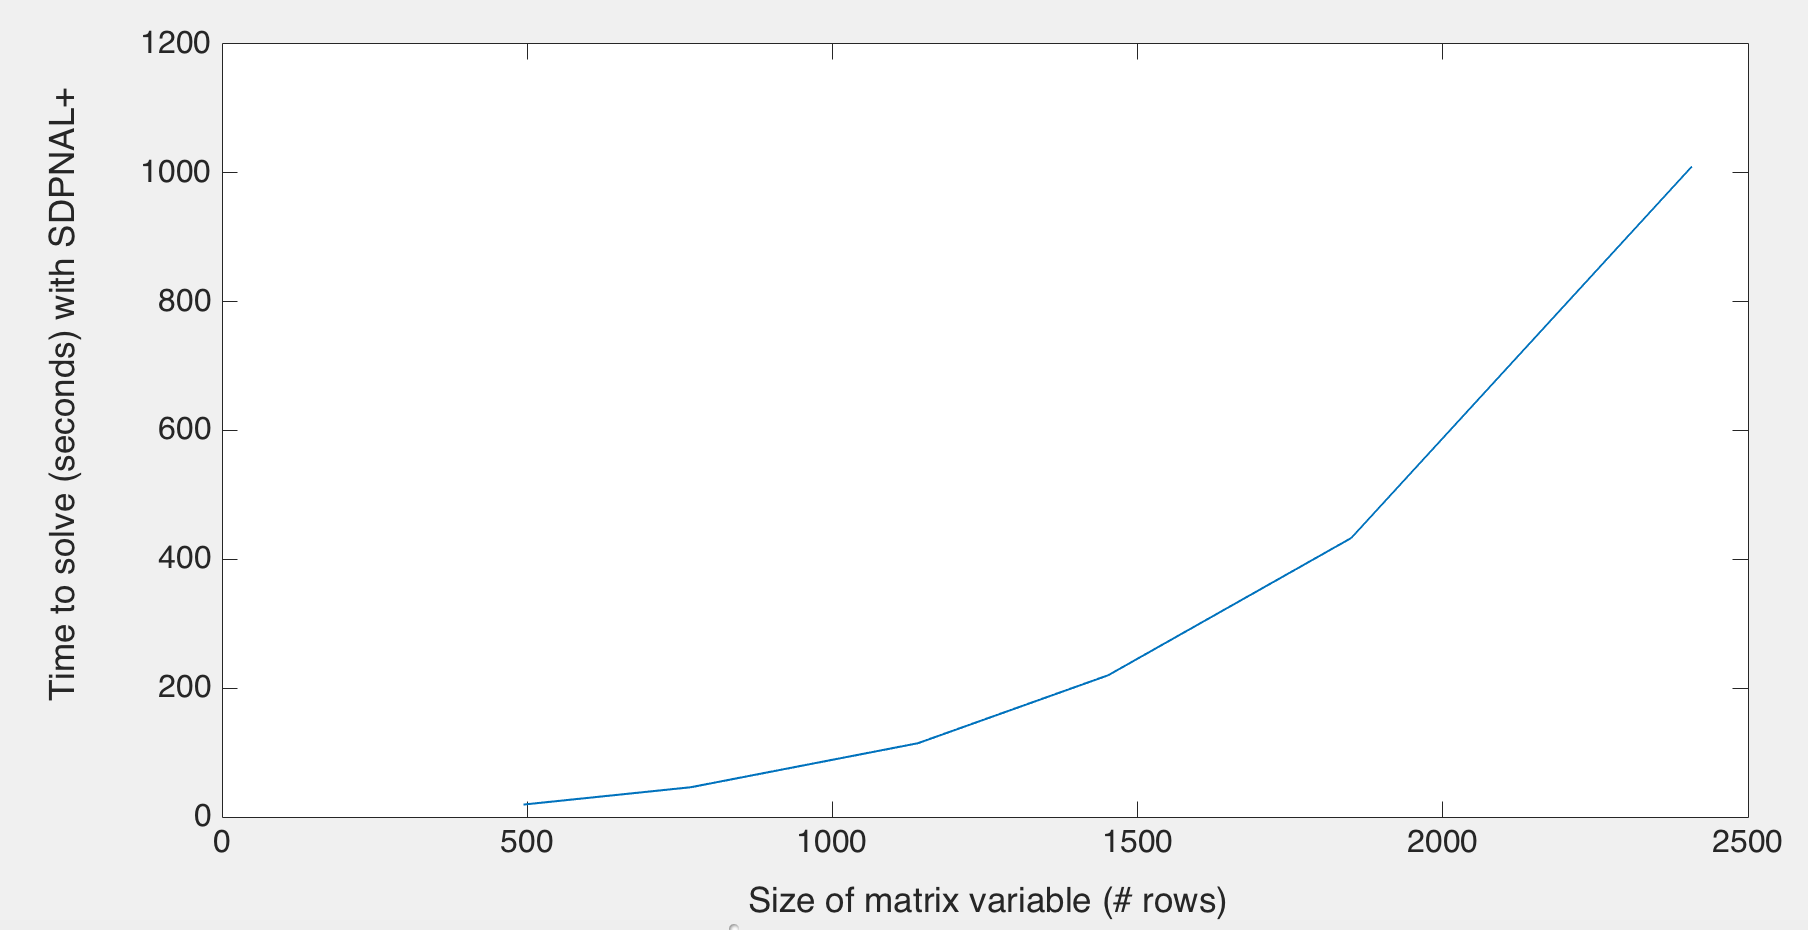
\includegraphics[width=\textwidth]{images/runtime}
\end{figure}

\section{Experimental Results}

We conducted empirical testing on two different CSPs to evaluate and compare the performance of SDP vector clustering and the Variable Folding Method. We also performed sensitivity testing on the Variable Folding Method with respect to the parameter $\epsilon$, which determines the spacing of the $\epsilon$-net, and to the domain size.

The first CSP is the Americas problem, a graph coloring problem (i.e. max-cut) where the graph is a map of North and South America with the countries rendered as nodes and borders as edges. The CSP contains 24 variables and 38 constraints, which is a small enough size that it can be solved exactly using Gurobi. We solved this problem with domains of 2, 3, and 4 colors in three different ways: exactly, using SDP vector clustering, and using the Variable Folding Method. The results are shown in \autoref{americas}. First, we are interested in how much the Variable Folding Method is able to reduce the size of the problem. In \autoref{americas-reduction}, we can see that the reduction in variables depends on both domain size and $\epsilon$, with domain size having the larger impact. The number of variables cannot be reduced at all when the domain size is 4, and $\epsilon$ has little effect for a domain size of 3. In the best case, with domain 2 and a large $\epsilon$, the number of variables can be reduced by over 40\%. Next we are interested in the solution quality with SDP vector clustering and the Variable Folding Method, relative to each other and to the optimal solution. These plots are also contained in \autoref{americas}. Note that 2- and 3-colorings of this graph are not satisfiable, but the y-axis of all the solution plots has been normalized so that the optimal solution is 1. We observe that the Variable Folding Method is closest to the optimal solution in all three plots. The difference is 4\% in \ref{2-coloring}, and Variable Folding Method has the optimal solution in \ref{3-coloring} and \ref{4-coloring}. The best result achieved by SDP vector clustering in \ref{4-coloring} is a 25\% difference.

\begin{figure}[ht!]
\centering
	\begin{subfigure}[b]{0.45\textwidth}
	\centering
	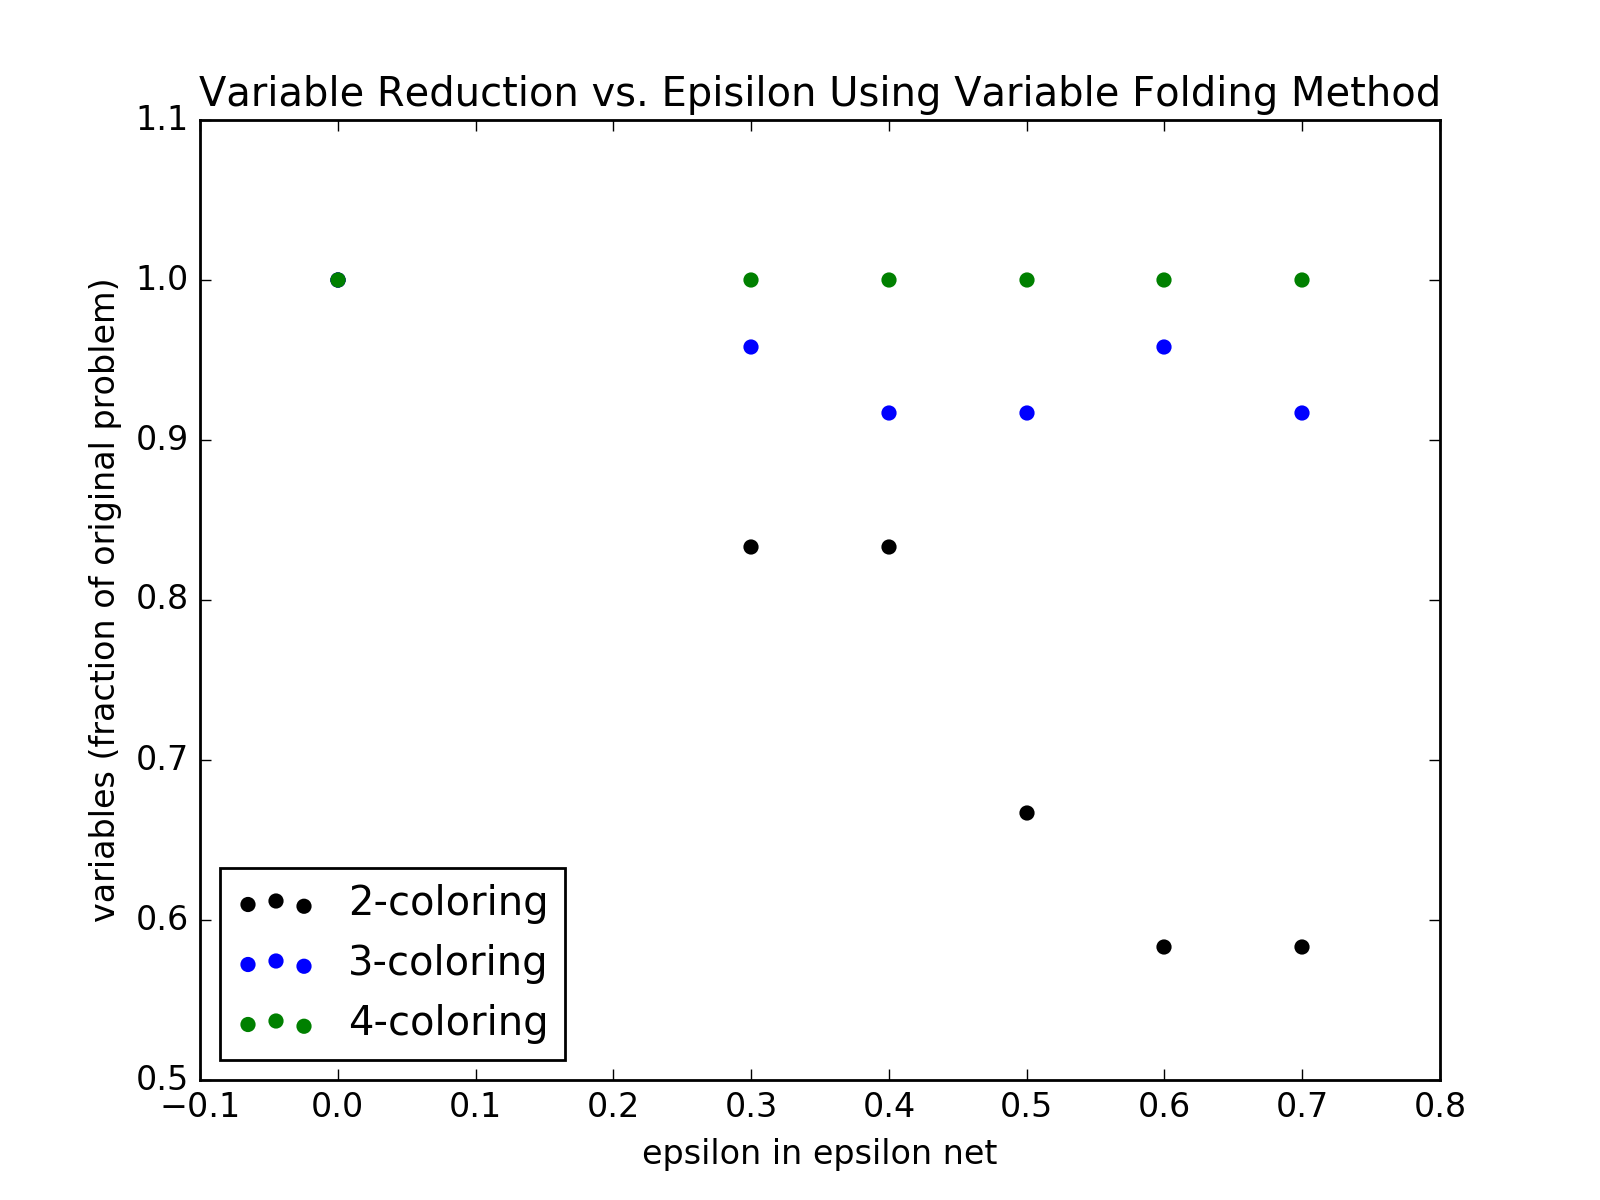
\includegraphics[width=\textwidth]{variables_epsilon_americas}
	\caption{Reduction in variables with variable folding method vs. epsilon and domain}
	\label{americas-reduction}
	\end{subfigure}
	~
	\begin{subfigure}[b]{0.45\textwidth}
	\centering
	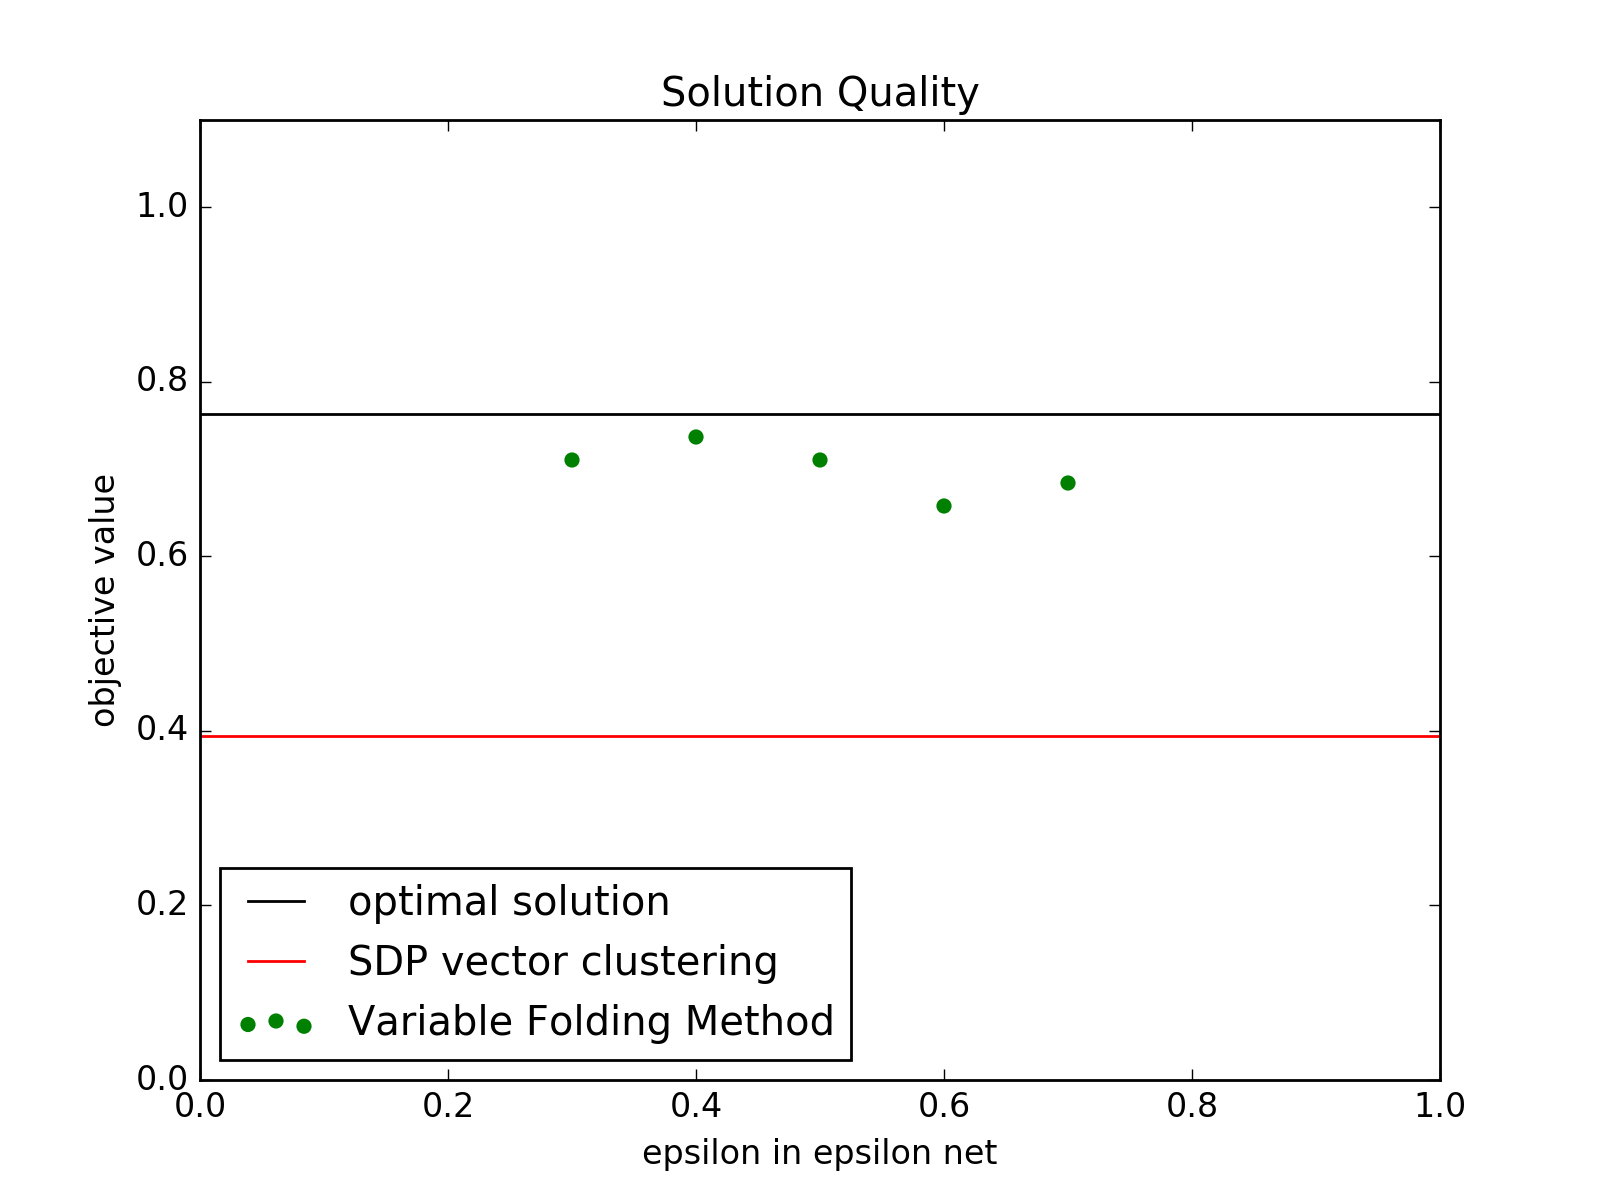
\includegraphics[width=\textwidth]{solution_epsilon_2coloring}
	\caption{Solution quality for 2-coloring the Americas}
	\label{2-coloring}
	\end{subfigure}

	\begin{subfigure}[b]{0.45\textwidth}
	\centering
	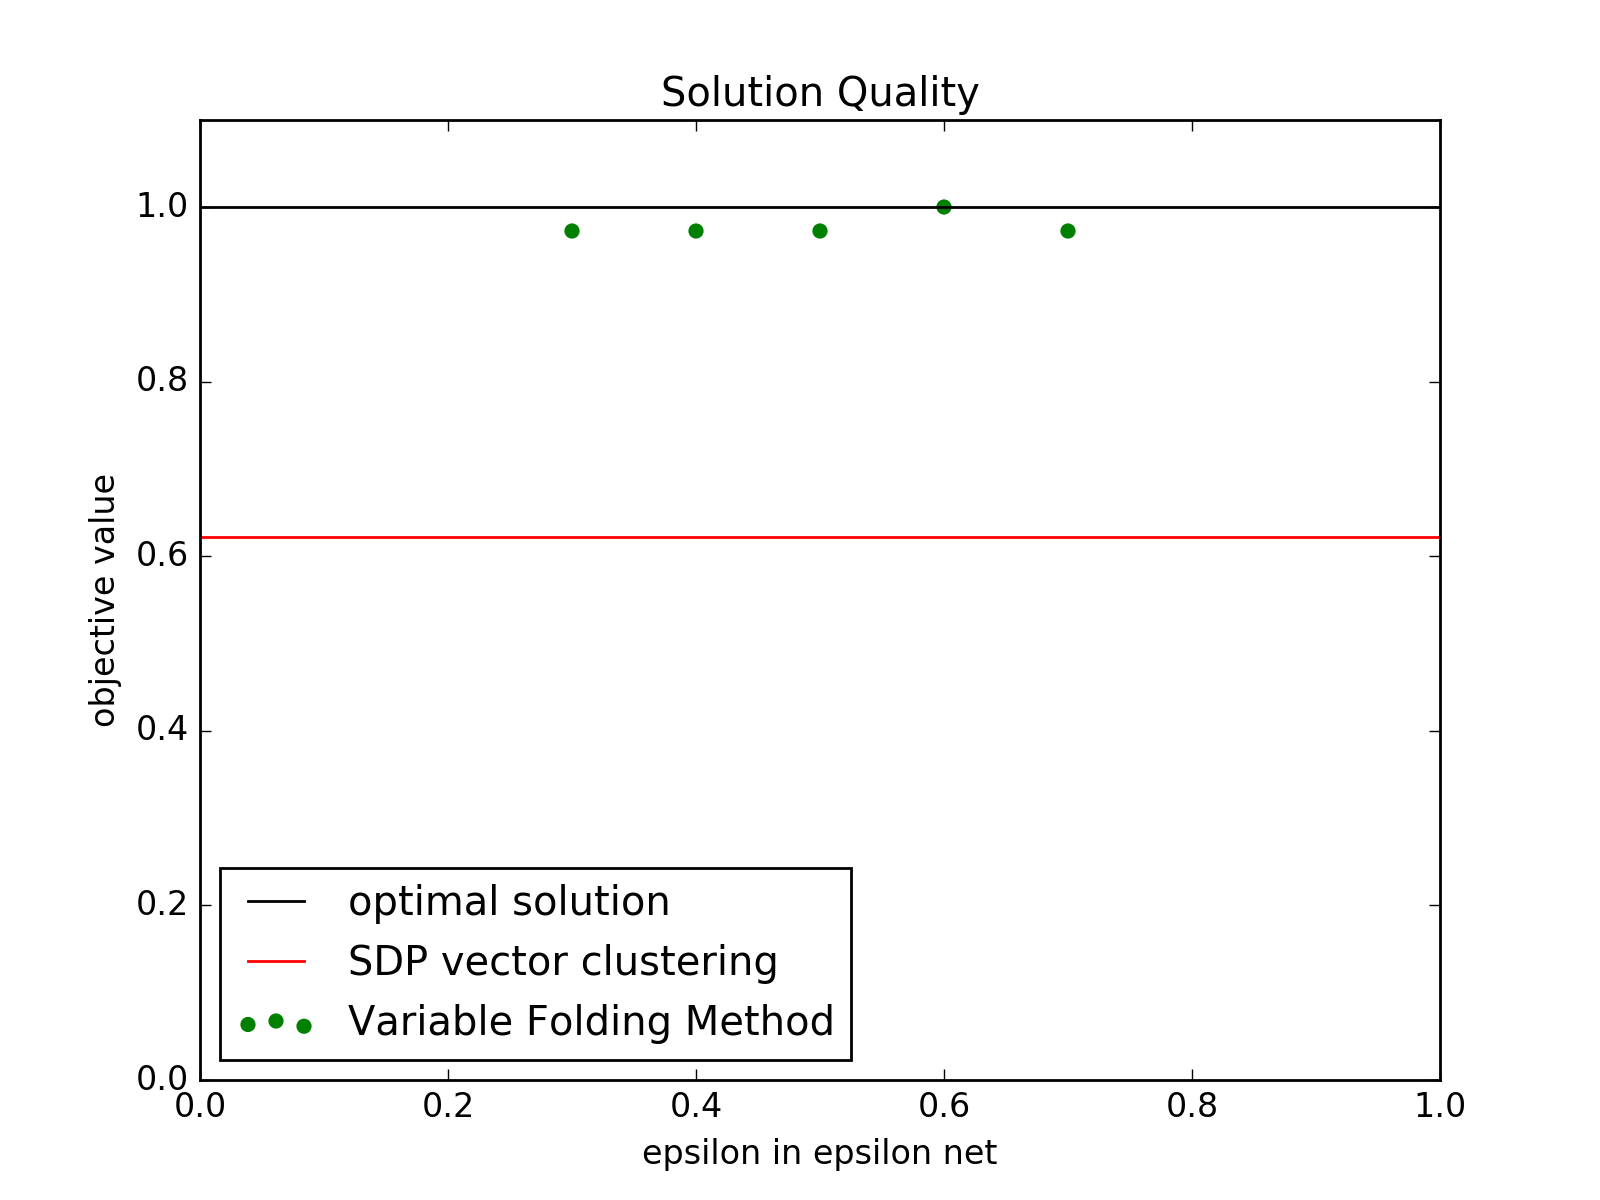
\includegraphics[width=\textwidth]{solution_epsilon_3coloring}
	\caption{Solution quality for 3-coloring the Americas}
	\label{3-coloring}
	\end{subfigure}
	~
	\begin{subfigure}[b]{0.45\textwidth}
	\centering
	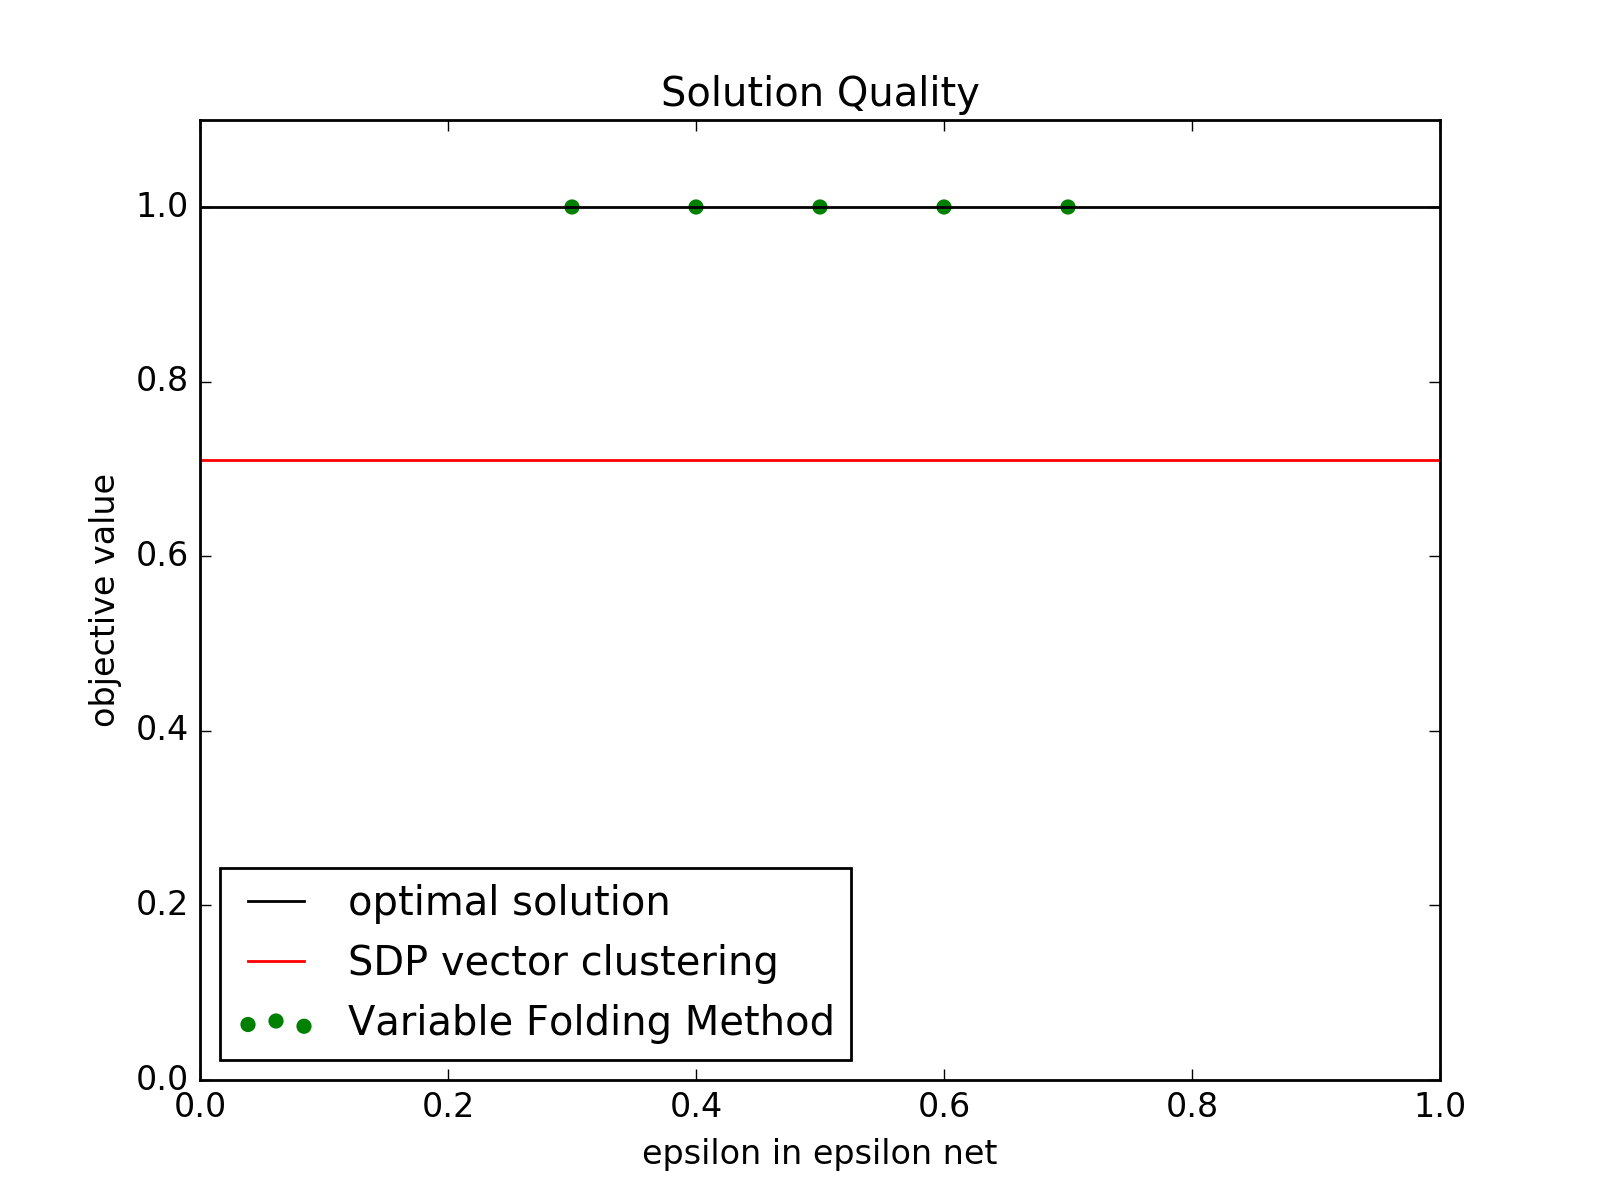
\includegraphics[width=\textwidth]{solution_epsilon_4coloring}
	\caption{Solution quality for 4-coloring the Americas}
	\label{4-coloring}
	\end{subfigure}
\caption{Evaluation of SDP Vector Clustering and the Variable Folding Method on the Americas Graph-Coloring Problem}
\label{americas}
\end{figure}
\FloatBarrier
The second CSP is the pigeonhole problem, a SAT problem where the objective is to place items in boxes without having more than 1 item in the same box. All of the instances tested are not satisfiable (more items than boxes) but are still interesting as a test of our method for solving CSPs. Even an approximation algorithm should be able to identify (1) that not all constraints can be satisfied and (2) how many constraints can be satisfied. We limited ourselves to instances that were small enough to solve exactly. The largest instance presented here (11 items in 9 boxes) has 572 constraints, 165 variables and an arity of 2, for $numConstraints |D|^{arity} + numVariables |D|=$4,906 integer variables in Gurobi. The figures are similar to those presented for the Americas problem. In \autoref{pigeon-reduction}, only $\epsilon$ varies, not the domain. We see that the Variable Folding Method can eliminate more variables the larger the problem gets, with a reduction of over 80\% possible with large $\epsilon$ for 10 items in 8 boxes and 11 items in 9 boxes. Even with small $\epsilon$, the number of variables is reduced by 50\% in the largest problems. In the solution quality plots, we see that the Variable Folding Method achieves or is very close to the optimal solution, with a slight degradation in solution quality as $\epsilon$ increases. SDP vector clustering is not close to the optimal solution, although the approximation error improves from about 30\% in \ref{n6m4} to 15\% in \ref{n11m9} as the problem size grows.

\begin{figure}[ht!]
\centering
	\begin{subfigure}[b]{0.45\textwidth}
	\centering
	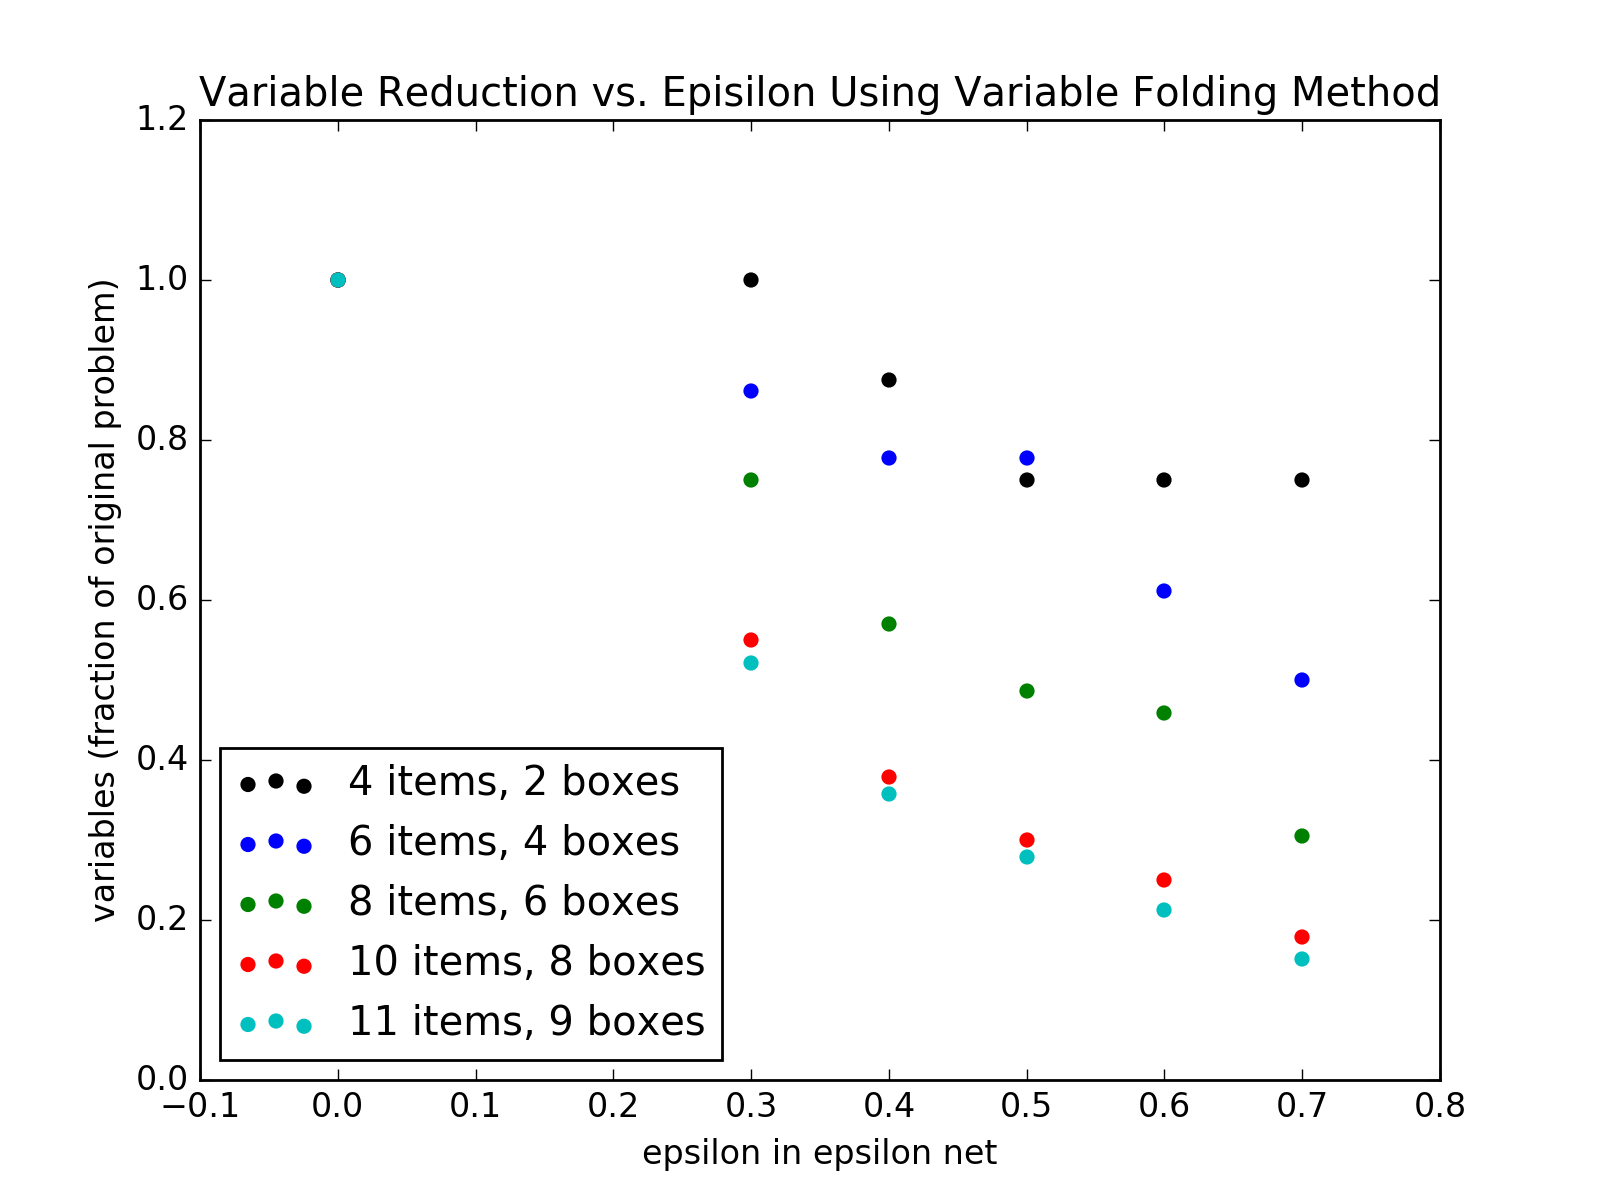
\includegraphics[width=\textwidth]{variables_epsilon_pigeon}
	\caption{Reduction in variables with variable folding method vs. epsilon and domain}
	\label{pigeon-reduction}
	\end{subfigure}
	~
	\begin{subfigure}[b]{0.45\textwidth}
	\centering
	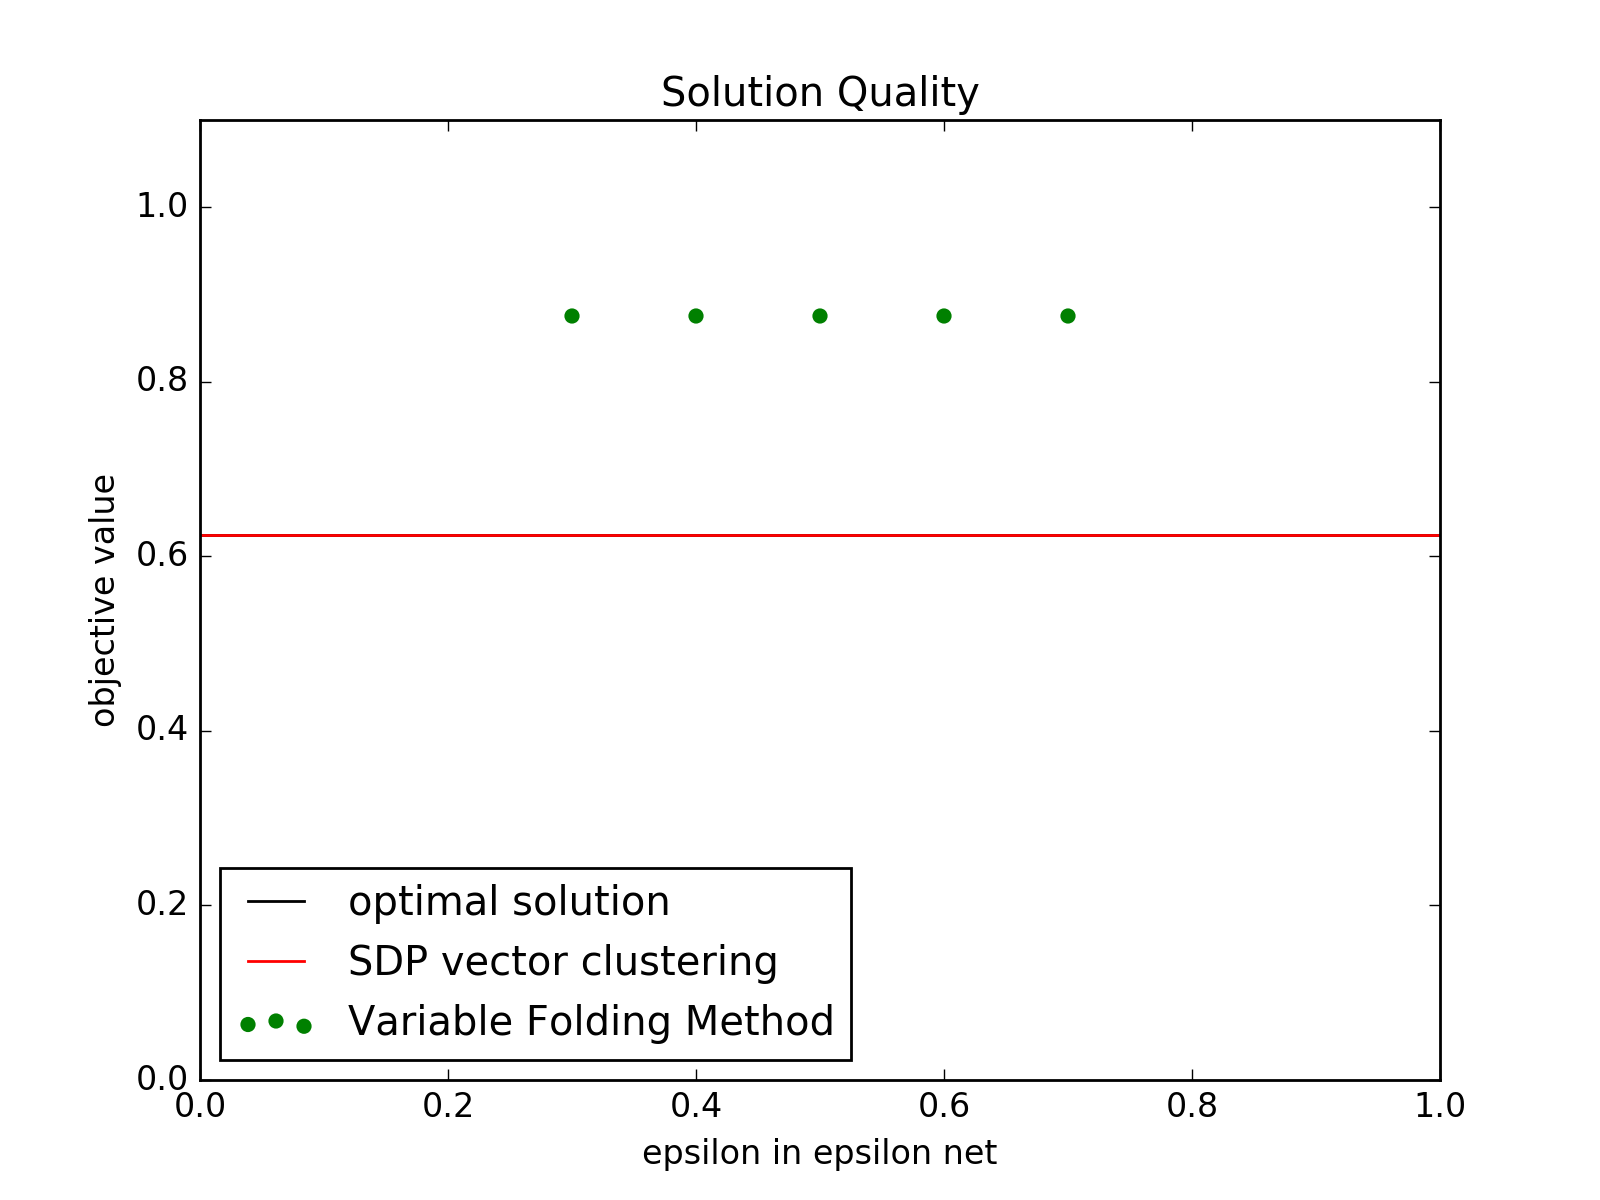
\includegraphics[width=\textwidth]{solution_epsilon_n4m2}
	\caption{Solution quality for 4 items in 2 boxes}
	\label{n4m2}
	\end{subfigure}

	\begin{subfigure}[b]{0.45\textwidth}
	\centering
	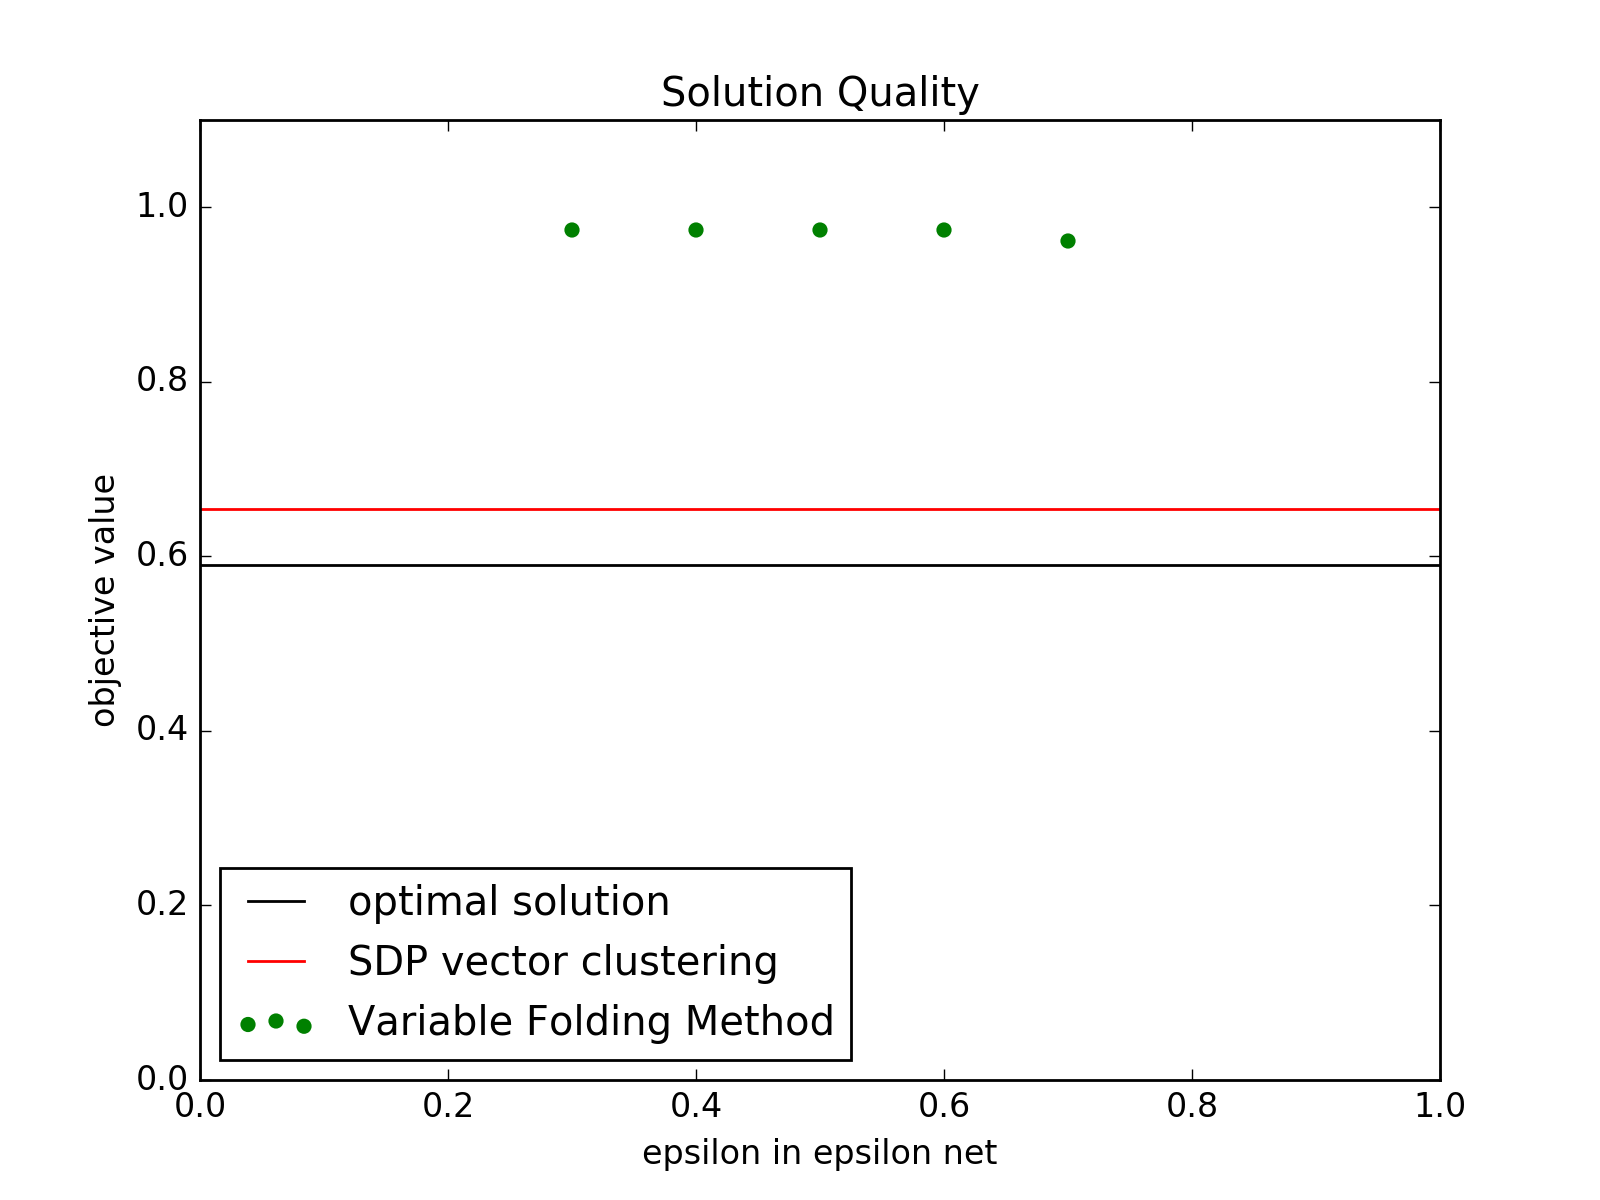
\includegraphics[width=\textwidth]{solution_epsilon_n6m4}
	\caption{Solution quality for 6 items in 4 boxes}
	\label{n6m4}
	\end{subfigure}
	~
	\begin{subfigure}[b]{0.45\textwidth}
	\centering
	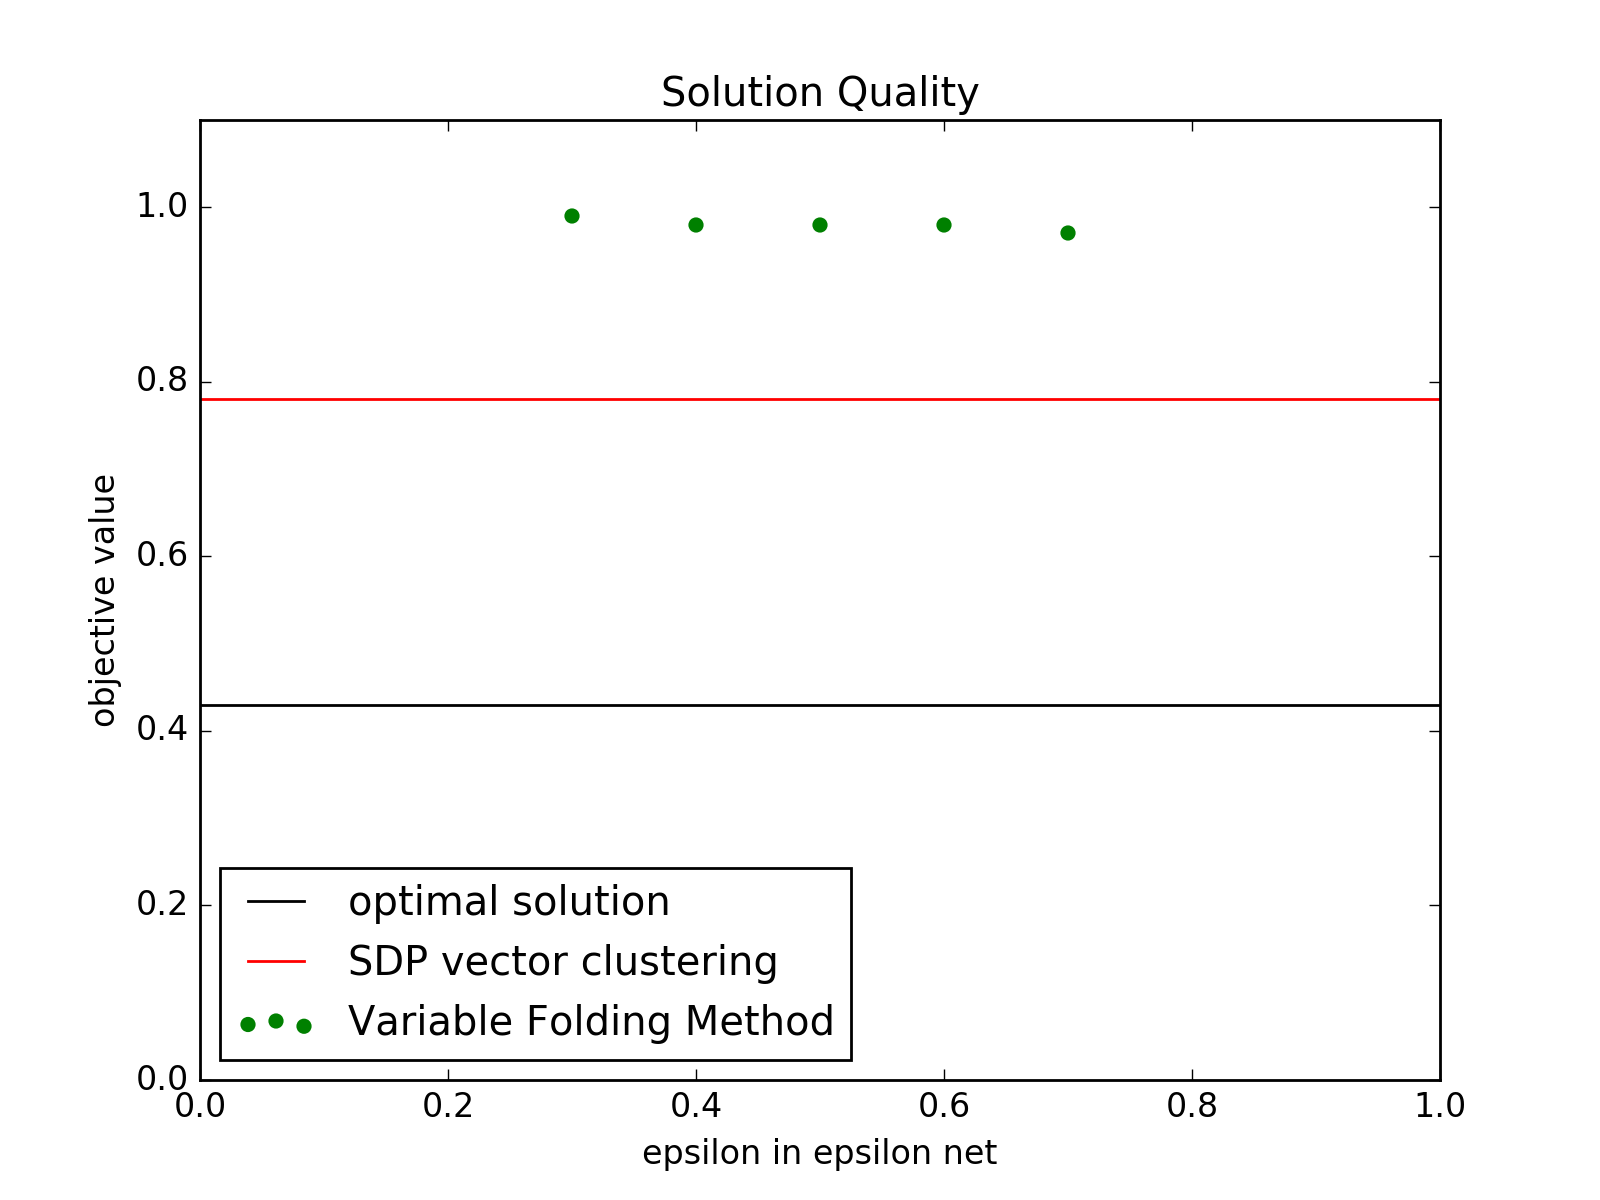
\includegraphics[width=\textwidth]{solution_epsilon_n8m6}
	\caption{Solution quality for 8 items in 6 boxes}
	\label{n8m6}
	\end{subfigure}

	\begin{subfigure}[b]{0.45\textwidth}
	\centering
	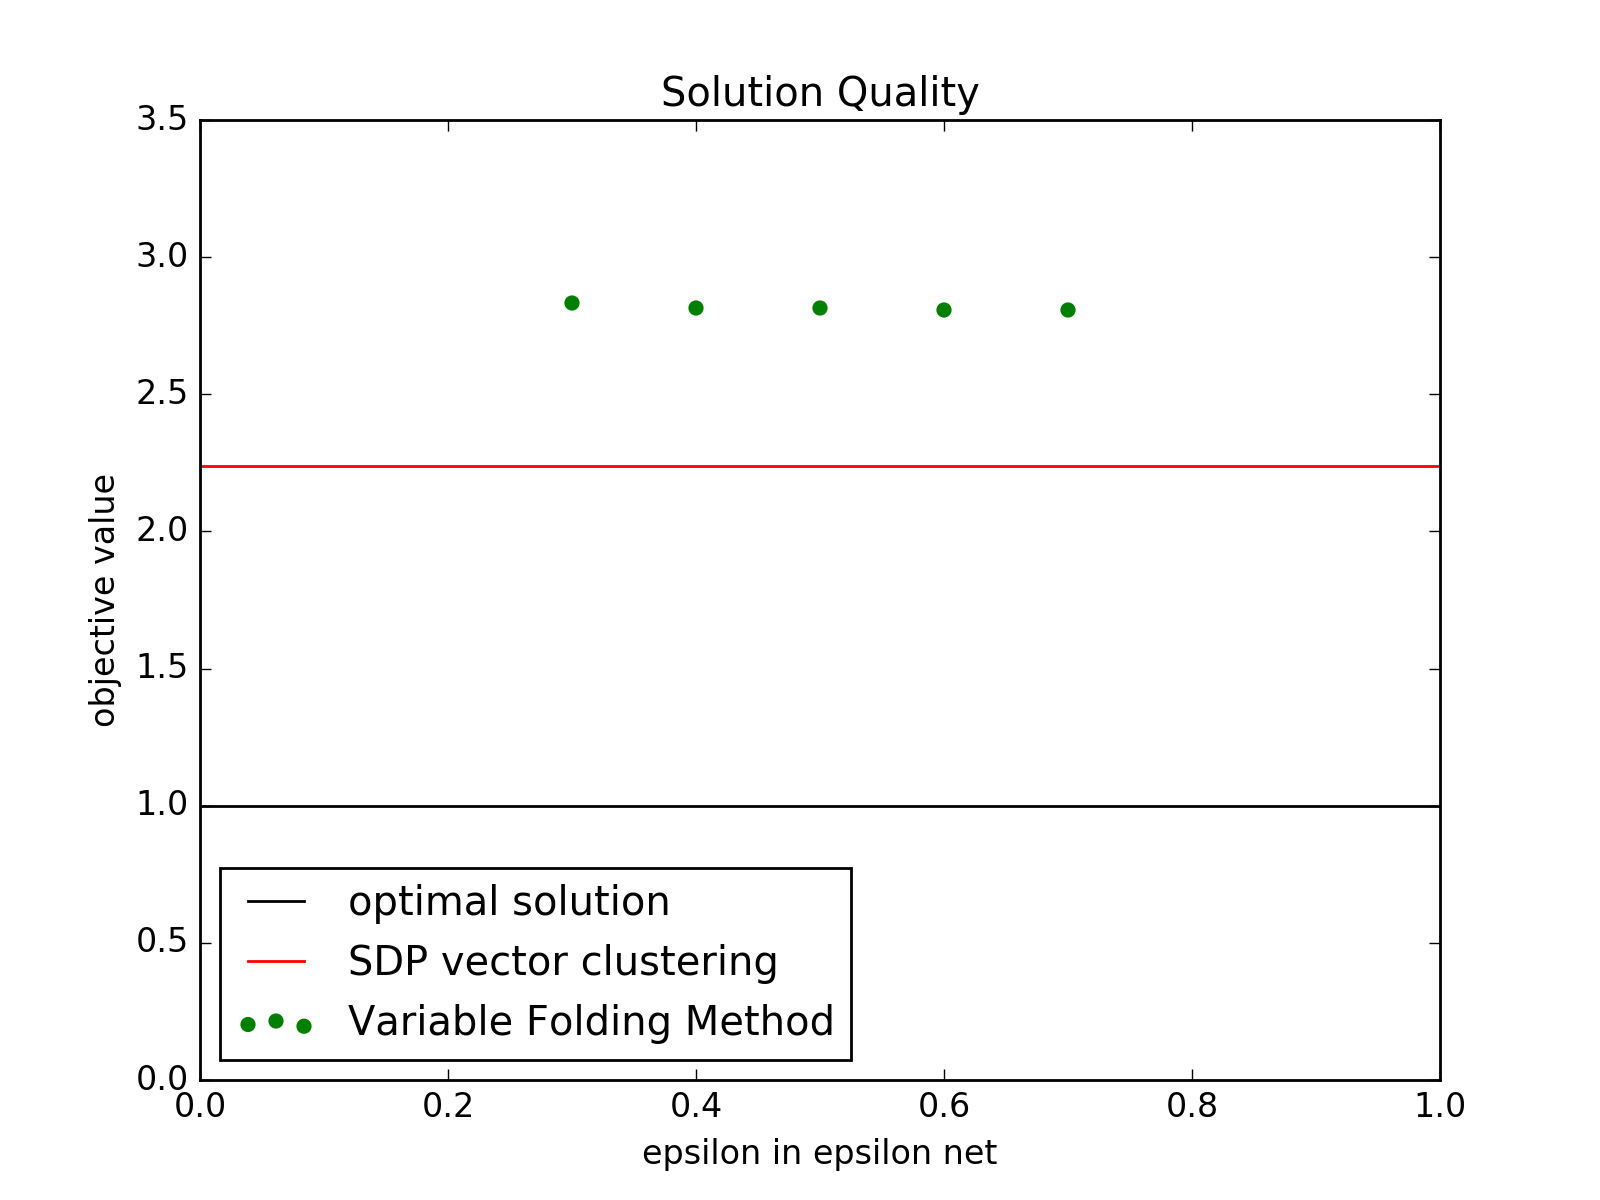
\includegraphics[width=\textwidth]{solution_epsilon_n10m8}
	\caption{Solution quality for 10 items in 8 boxes}
	\label{n10m8}
	\end{subfigure}
	~
	\begin{subfigure}[b]{0.45\textwidth}
	\centering
	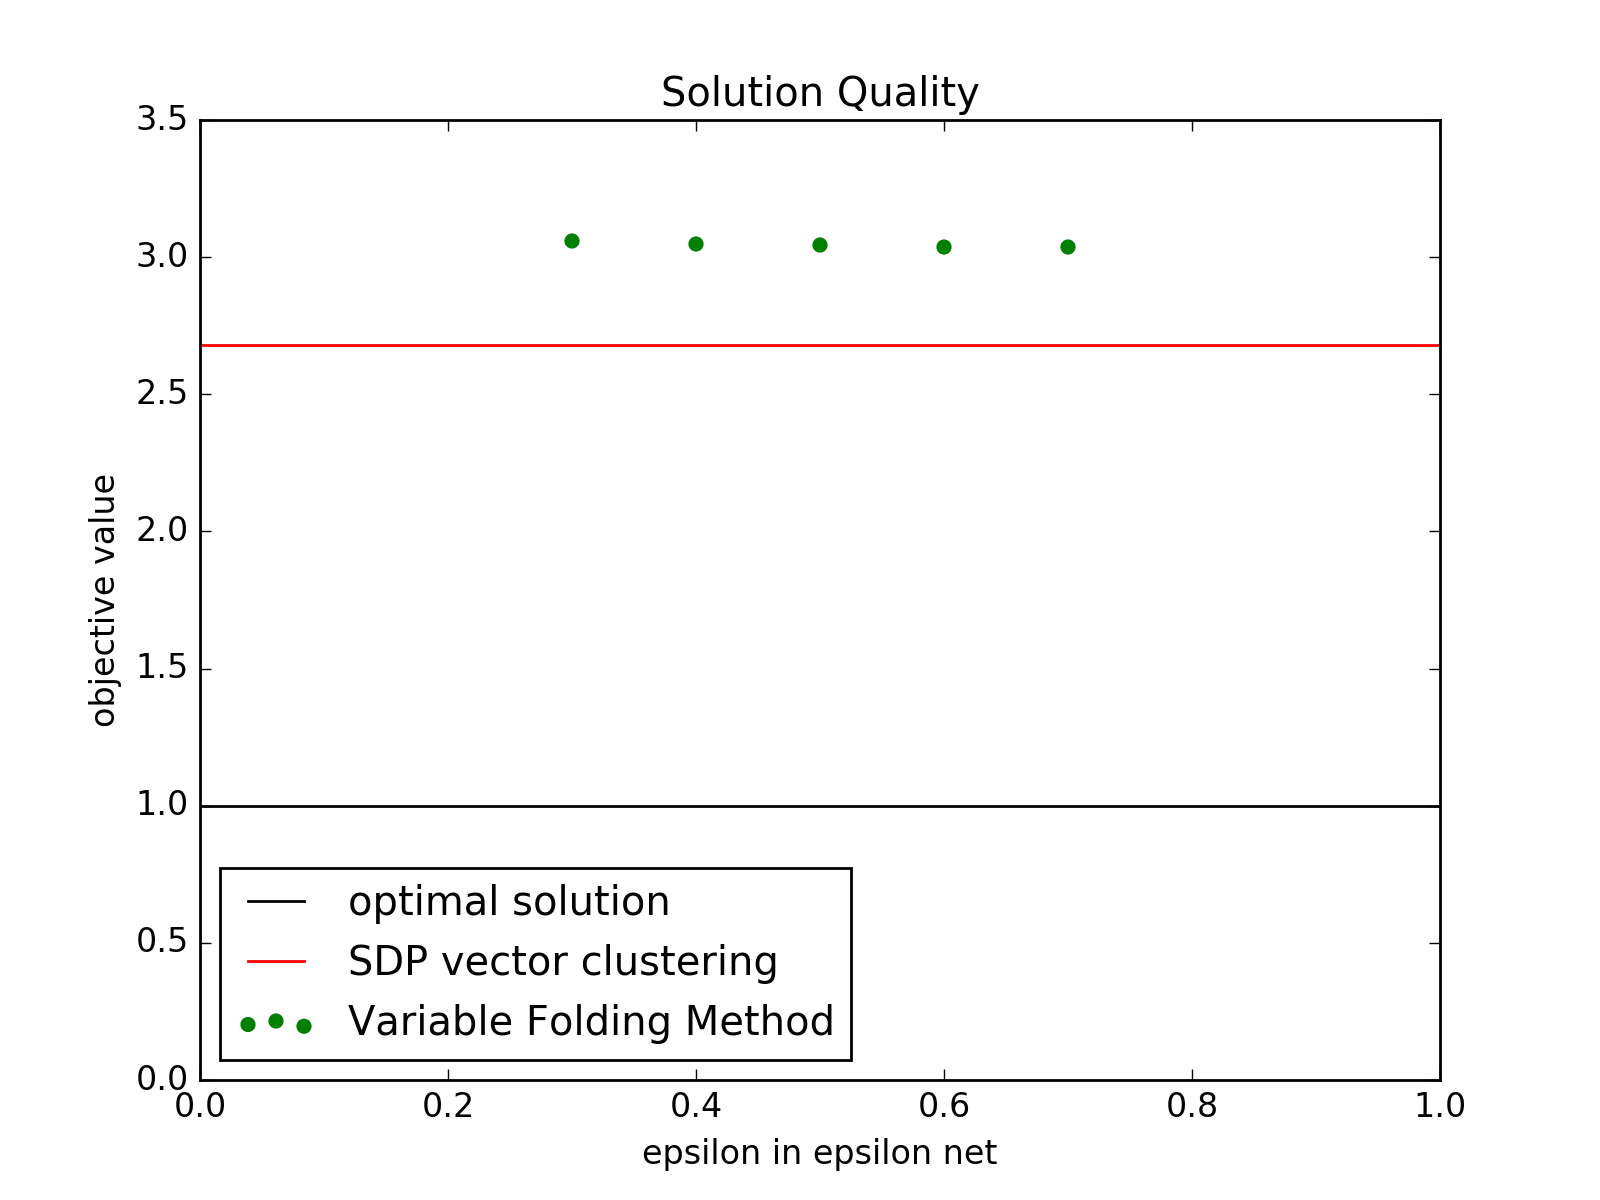
\includegraphics[width=\textwidth]{solution_epsilon_n11m9}
	\caption{Solution quality for 11 items in 9 boxes}
	\label{n11m9}
	\end{subfigure}
\caption{Evaluation of SDP Vector Clustering and the Variable Folding Method on the Pigeonhole Problem}
\label{pigeon}
\end{figure}

\section{Conclusion}

In this work, we developed a Matlab-based software package for solving CSP's. This package takes a CSP, computes the basic SDP relaxation, and feeds the inputs to SDPNAL+, a powerful solver that can handle large scale problems. Once the SDP solution is found, we need to convert it to an assignment of variables for the CSP. This is done using two heuristics: SDP vector clustering and an approximation of the Variable Folding Method. We used an approximation of the Variable Folding Method because the published method, while polynomial, is impossibly large. We avoided this problem by projecting the SDP vectors onto $\mathbb{R}^2$, which greatly reduced the number of variables in the folded CSP. We then tested this software package on small graph coloring and pigeonhole problems, comparing the assignment heuristics to the exact solution . The Variable Folding Method, even with our approximation, proved to be very close to the optimal solution. SDP vector clustering, on the other hand, showed a fairly large approximation error in the two problems.

The two problems used to evaluate SDP vector clustering and the Variable Folding Method are favorable cases for SDP vector clustering because there are no constraints that reference specific values in the domain. In graph coloring, we simply want adjacent nodes to be different colors, and in the pigeonhole problem we want each box to contain no more than one item. If, for example, we wanted one node to be a particular color, or for one item to go in a specific box, then the assignment would affect the CSP objective. In the problems we tested, only the clustering process affects the CSP objective, not the assignment of values. If the assignment matters, then it is necessary to test all $|D|!$ possible assignments and the clustering method would be slower as a result.

We encountered various issues related to scaling in this work. Because SDPNAL+ is not supported by any general purpose modeling language, we had to construct the basic SDP relaxation ourselves. In large CSP's, the constraint matrices have millions of rows and columns, which created a large memory bottleneck. We identified and removed these issues using Matlab's Code Profiler. Another issue is that the Variable Folding Method depends on solving the folded problem exactly. Using the published version of this method which projects onto a random subspace in $\mathbb{R}^\beta$, we would end up with folded problems that are too large to solve exactly. Our approximation of projecting onto $\mathbb{R}^2$ instead helped to keep the folded problems small enough to solve exactly.

%references
\renewcommand{\bibname}{References}
\bibliographystyle{apalike}
\bibliography{./227c_references}

\end{document}
